\subsection{Investigation of new system model: Test of component models} \label{app:tj_2}
The model in the report carries with it some misfits wrt. connecting the entire system. It is well illustrated in \cref{fig:Block_diagram_inout}, where the red variables has to be input as constant inputs in order to simulate the system. For convenience, \cref{fig:Block_diagram_inout} is included here as well, in \cref{fig:Block_diagram_inout2}.
\begin{figure}[h!]
	\centering
	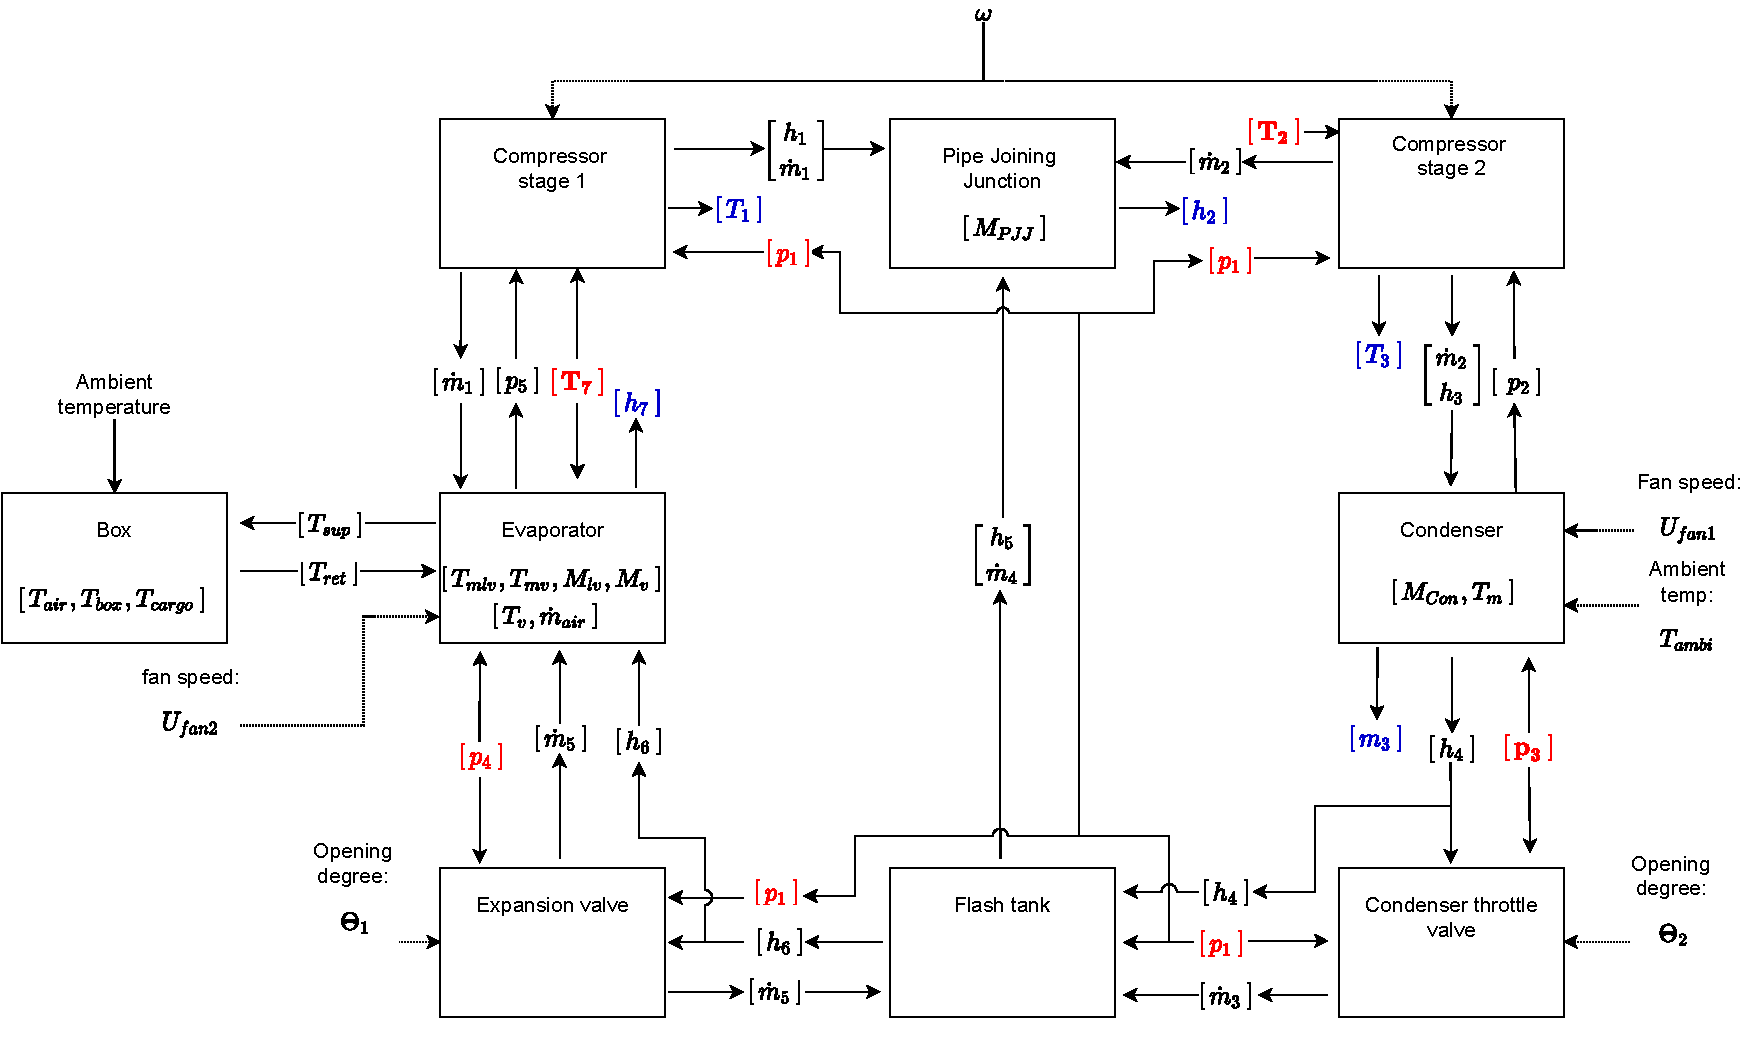
\includegraphics[width=1\textwidth]{Graphics/Block_Diagram_inout_flowValveVersion.pdf}
	\caption{Block diagram of input/output relationship of interface variables. Same as \cref{fig:Block_diagram_inout}. This block diagram is the the version currently documented in the report, and it has several issues.}
	\label{fig:Block_diagram_inout2}
\end{figure}

An obvious problem is the choice of having too many flow setting components. An example follows: The condenser throttle valve in \cref{fig:Block_diagram_inout2} is setting a flow, as is the compressor stage 2. This results in two misaligned flows that are not connected, and such, the Mass balance in the condenser is rigged, where $ M_{con} $ is deemed to integrate indefinitely if the perfect pressure $ p_3 $ is not found. This was exactly the case in the non linear model verification in \cref{fig:non_lin_sim_faulty_Mass}.

The choice of letting the valve being flow setting means that the non linear model can only be simulated in the chosen operating point for the constant inputs. It is desired to investigate the possibility of getting a more generic model that can approximate coupling effects in the refrigeration system, and without the need of external operating values for the red variables in \cref{fig:Block_diagram_inout}.

In order to omit the red external constant inputs, a reformulation of some of the components were necessary. This includes
\begin{enumerate}
	\item changing the valves from being flow setting to being pressure setting.
	\item changing the flash tank
	\item changing the pipe joining junction
	\item adding an extra state temperature state to the evaporator
	\item adding an extra pressure state in the condenser (has not been implemented yet).
\end{enumerate}

This results in a new block diagram that can be seen in \cref{fig:Block_diagram_inout_valvePres}

\begin{figure}[h!]
	\centering
	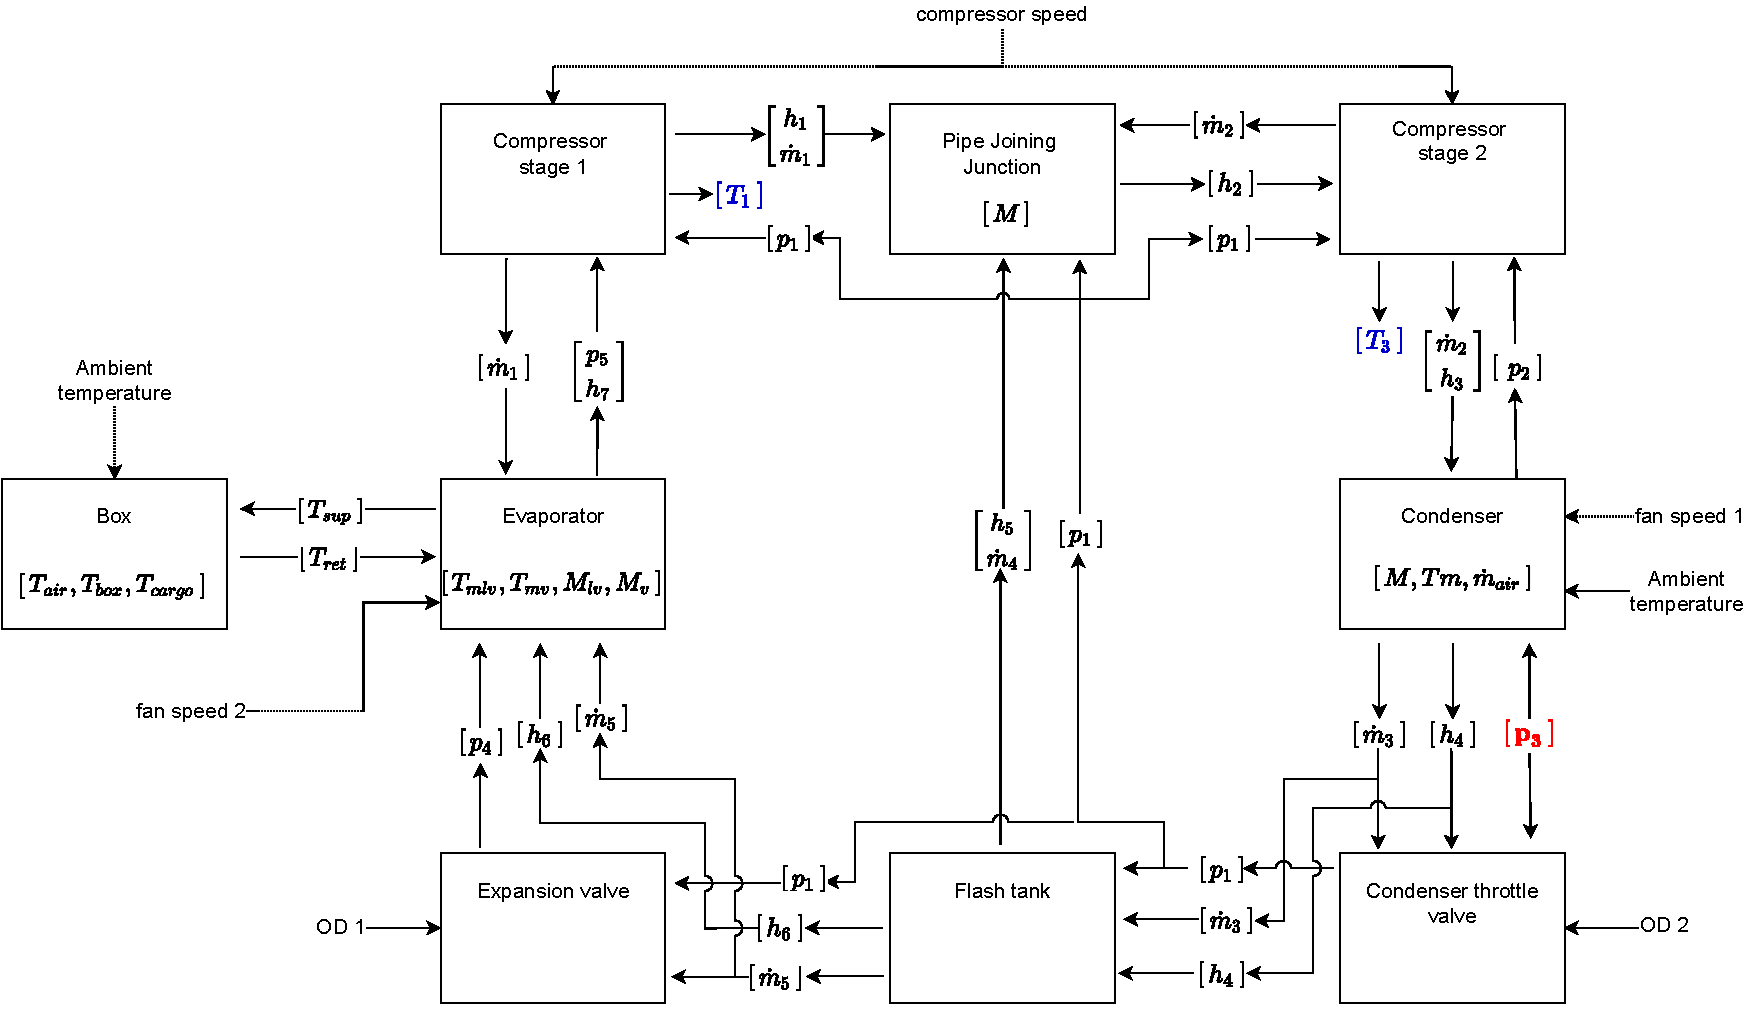
\includegraphics[width=1\textwidth]{Graphics/Block_Diagram_inout.pdf}
	\caption{Block diagram of input/output relationship of interface variables}
	\label{fig:Block_diagram_inout_valvePres}
\end{figure}

\subsubsection*{\textbf{Reformulation of components}}
The following section will cover reformulation of the component models that corresponds to \cref{fig:Block_diagram_inout_valvePres}.
\subsubsection*{Pressure setting valve model}

